\chapter{Особливості динамічних акустоіндукованих змін параметрів
кремнієвих діодів Шотки Mo$/n-n^+$--Si в широкому температурному інтервалі\label{Ch_USL_T_SD}}


%\begin{figure}[b]
%\center
%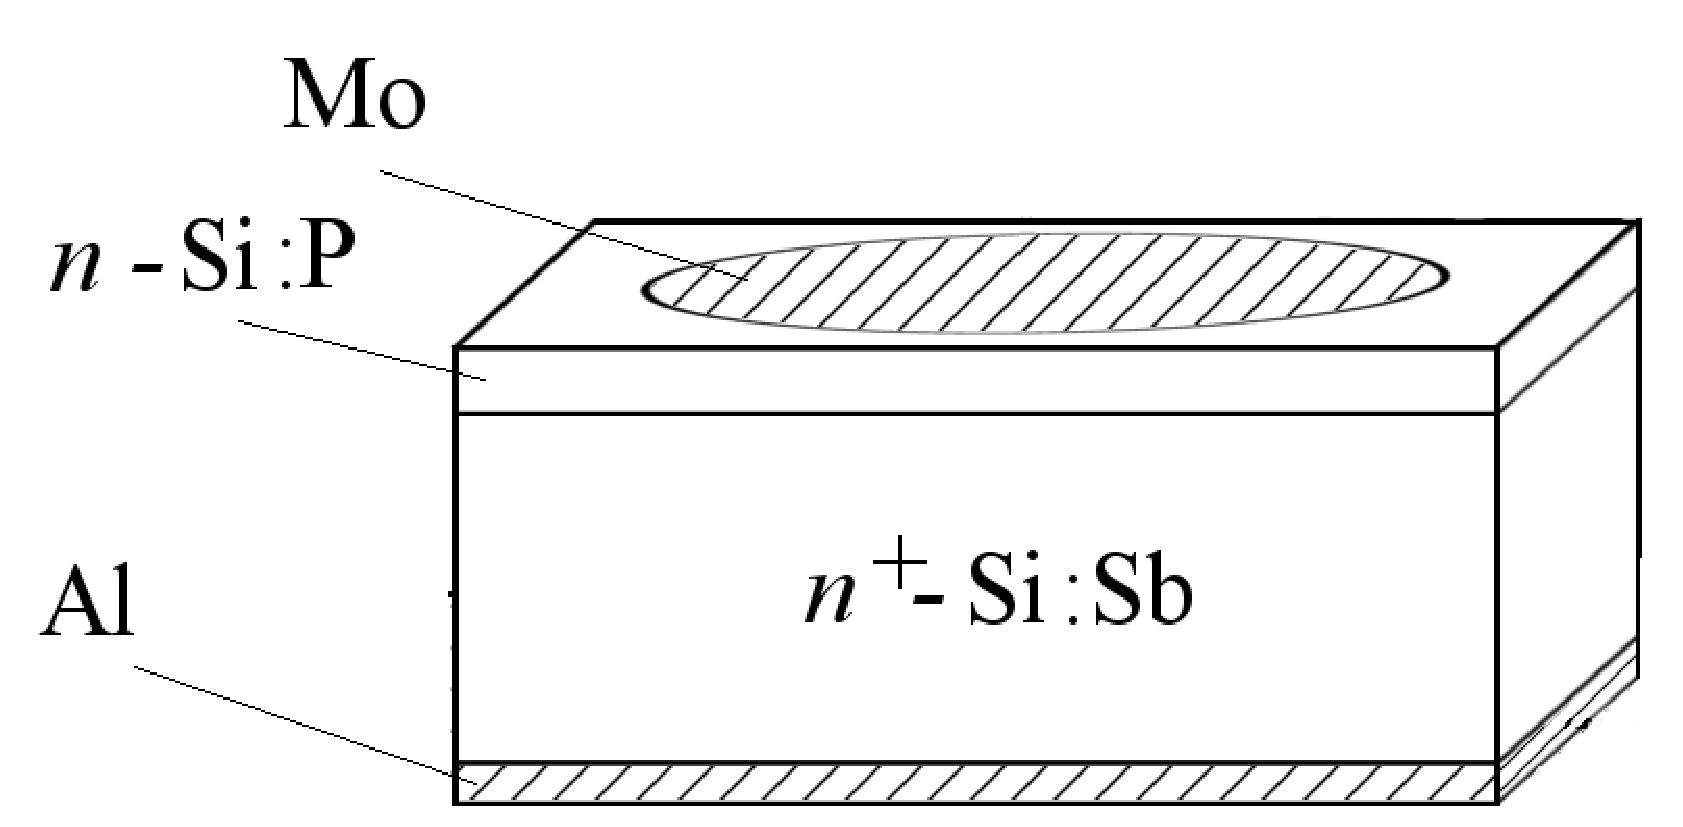
\includegraphics[width=0.65\textwidth]{MSSi}%
%\caption{\label{figMSSi}
%Структура зразків SSDA.
%}
%\end{figure}

%Для досліджень використовувалися діоди Шотки з наступною структурою:
%на підкладці $n^+$-Si:Sb (KЭС~0.01, товщина 250~мкм) знаходиться епітаксійний шар $n$-Si:P (товщина 0.2~мкм);
%на поверхні епі-шару створено контакт  Шотки діаметром 2 мм шляхом нанесення шару молібдену;
%на протилежному боці підкладки --- омічний контакт.

В дослідженнях використовувалися діоди Шотки, виготовлені на основі епітаксійної
структури $n$--$n^+$--Si.
Товщини епітаксійного шару та підкладки дорівнювали $0,2$~мкм та $250$~мкм, відповідно.
Епітаксійний шар був легований атомами фосфору, підкладка --- сурмою
(KЭС~0.01, концентрація вільних електронів $N_s\approx4,2\cdot10^{23}$~м$^{-3}$).
Для створення бар'єру на поверхню епітаксійного прошарку нанесено шар молібдену діаметром 2 мм (площа ДШ $A=3,14\cdot10^{-6}$~м$^2$).
З протилежного боку структури нанесено прошарок алюмінію, який забезпечував наявність омічного контакту.
Схематичне зображення структур наведено на Рис.~\ref{figMSSi}.
Структури виготовлені на <<Томилинском электронном заводе>>  (Росія), де вони використовуються при виробництві випрямляючих діодів, зокрема типу 2Д219.
Надалі для позначення зразків використовується скорочення SSDA.

%\begin{table}
%\caption{\label{tabMSSi}Параметри структур Mo$/n$--$n^+$--Si.
%}
%%\begin{tabular}{|c|c|c|c|}
%\begin{tabularx}{\textwidth}{|>{\centering\arraybackslash}X|>{\centering\arraybackslash}X|>{\centering\arraybackslash}X|>{\centering\arraybackslash}X|>{\centering\arraybackslash}X|}
%\hline
%$N_d$, м$^{-3}$&$N_s$, м$^{-3}$&$A$, м$^2$&Позначення\\
%\hline
%$(1,1\div1,3)\cdot10^{23}$&$4,2\cdot10^{23}$&$3,14\cdot10^{-6}$&SSDA\\
%\hline
%$7,25\cdot10^{21}$&$4,2\cdot10^{22}$&$49\cdot10^{-6}$&SSDB\\
%\hline
%\end{tabularx}
%\end{table}

\section{Особливості ультразвукового навантаження при низьких температурах\label{SSDB:USL}}


Наявність чи відсутність діелектричного прошарку визначалась особливостями вимірювання ВАХ.
Використання буфера дозволяло найефективніше мінімізувати вплив п'єзоперетворювача на процеси у напівпровіднику:
металевий буфер виконував роль як електричного, так і температурного екрану.
Тип схеми УЗН, яка використовувалася в тих чи інших дослідах, зазначено на початку відповідного розділу.

%Під час проведенні УЗН за схемами, наведеними на Рис.~\ref{figUSL},а  та Рис.~\ref{figUSL},б дослідження проводились у достатньо вузькому температурному діапазоні $290\div340$~К.
При цьому вважалось, що параметри п'зоелектричного перетворювача змінюються мало, сталість величини $V_\mathtt{RF}$ забезпечує незмінність $W_\mathtt{US}$  для всього діапазону температур, і для оцінки параметрів ультразвукового навантаження використовувалися формули
(\labelcref{eqAmpUS,eqWus,eqM0,eqDefUS}).
Вплив металевого екрануючого шару та діелектричного слюдяного прошарку на інтенсивність звуку, введеного в зразок, вважався знехтувано малим, так як їх товщина значно менша ніж половина довжини АХ.
%В той же час, подібні спрощення не є виправданими у випадку, коли коли використовується схема УЗН, показана на Рис.~\ref{figUSL},в і вимірювання проводяться в широкому температурному діапазоні.
%Більш детально процедура оцінки $W_\mathtt{US}$ в цьому випадку описана в наступному розділі \ref{subLowT}.


\begin{figure}
\center
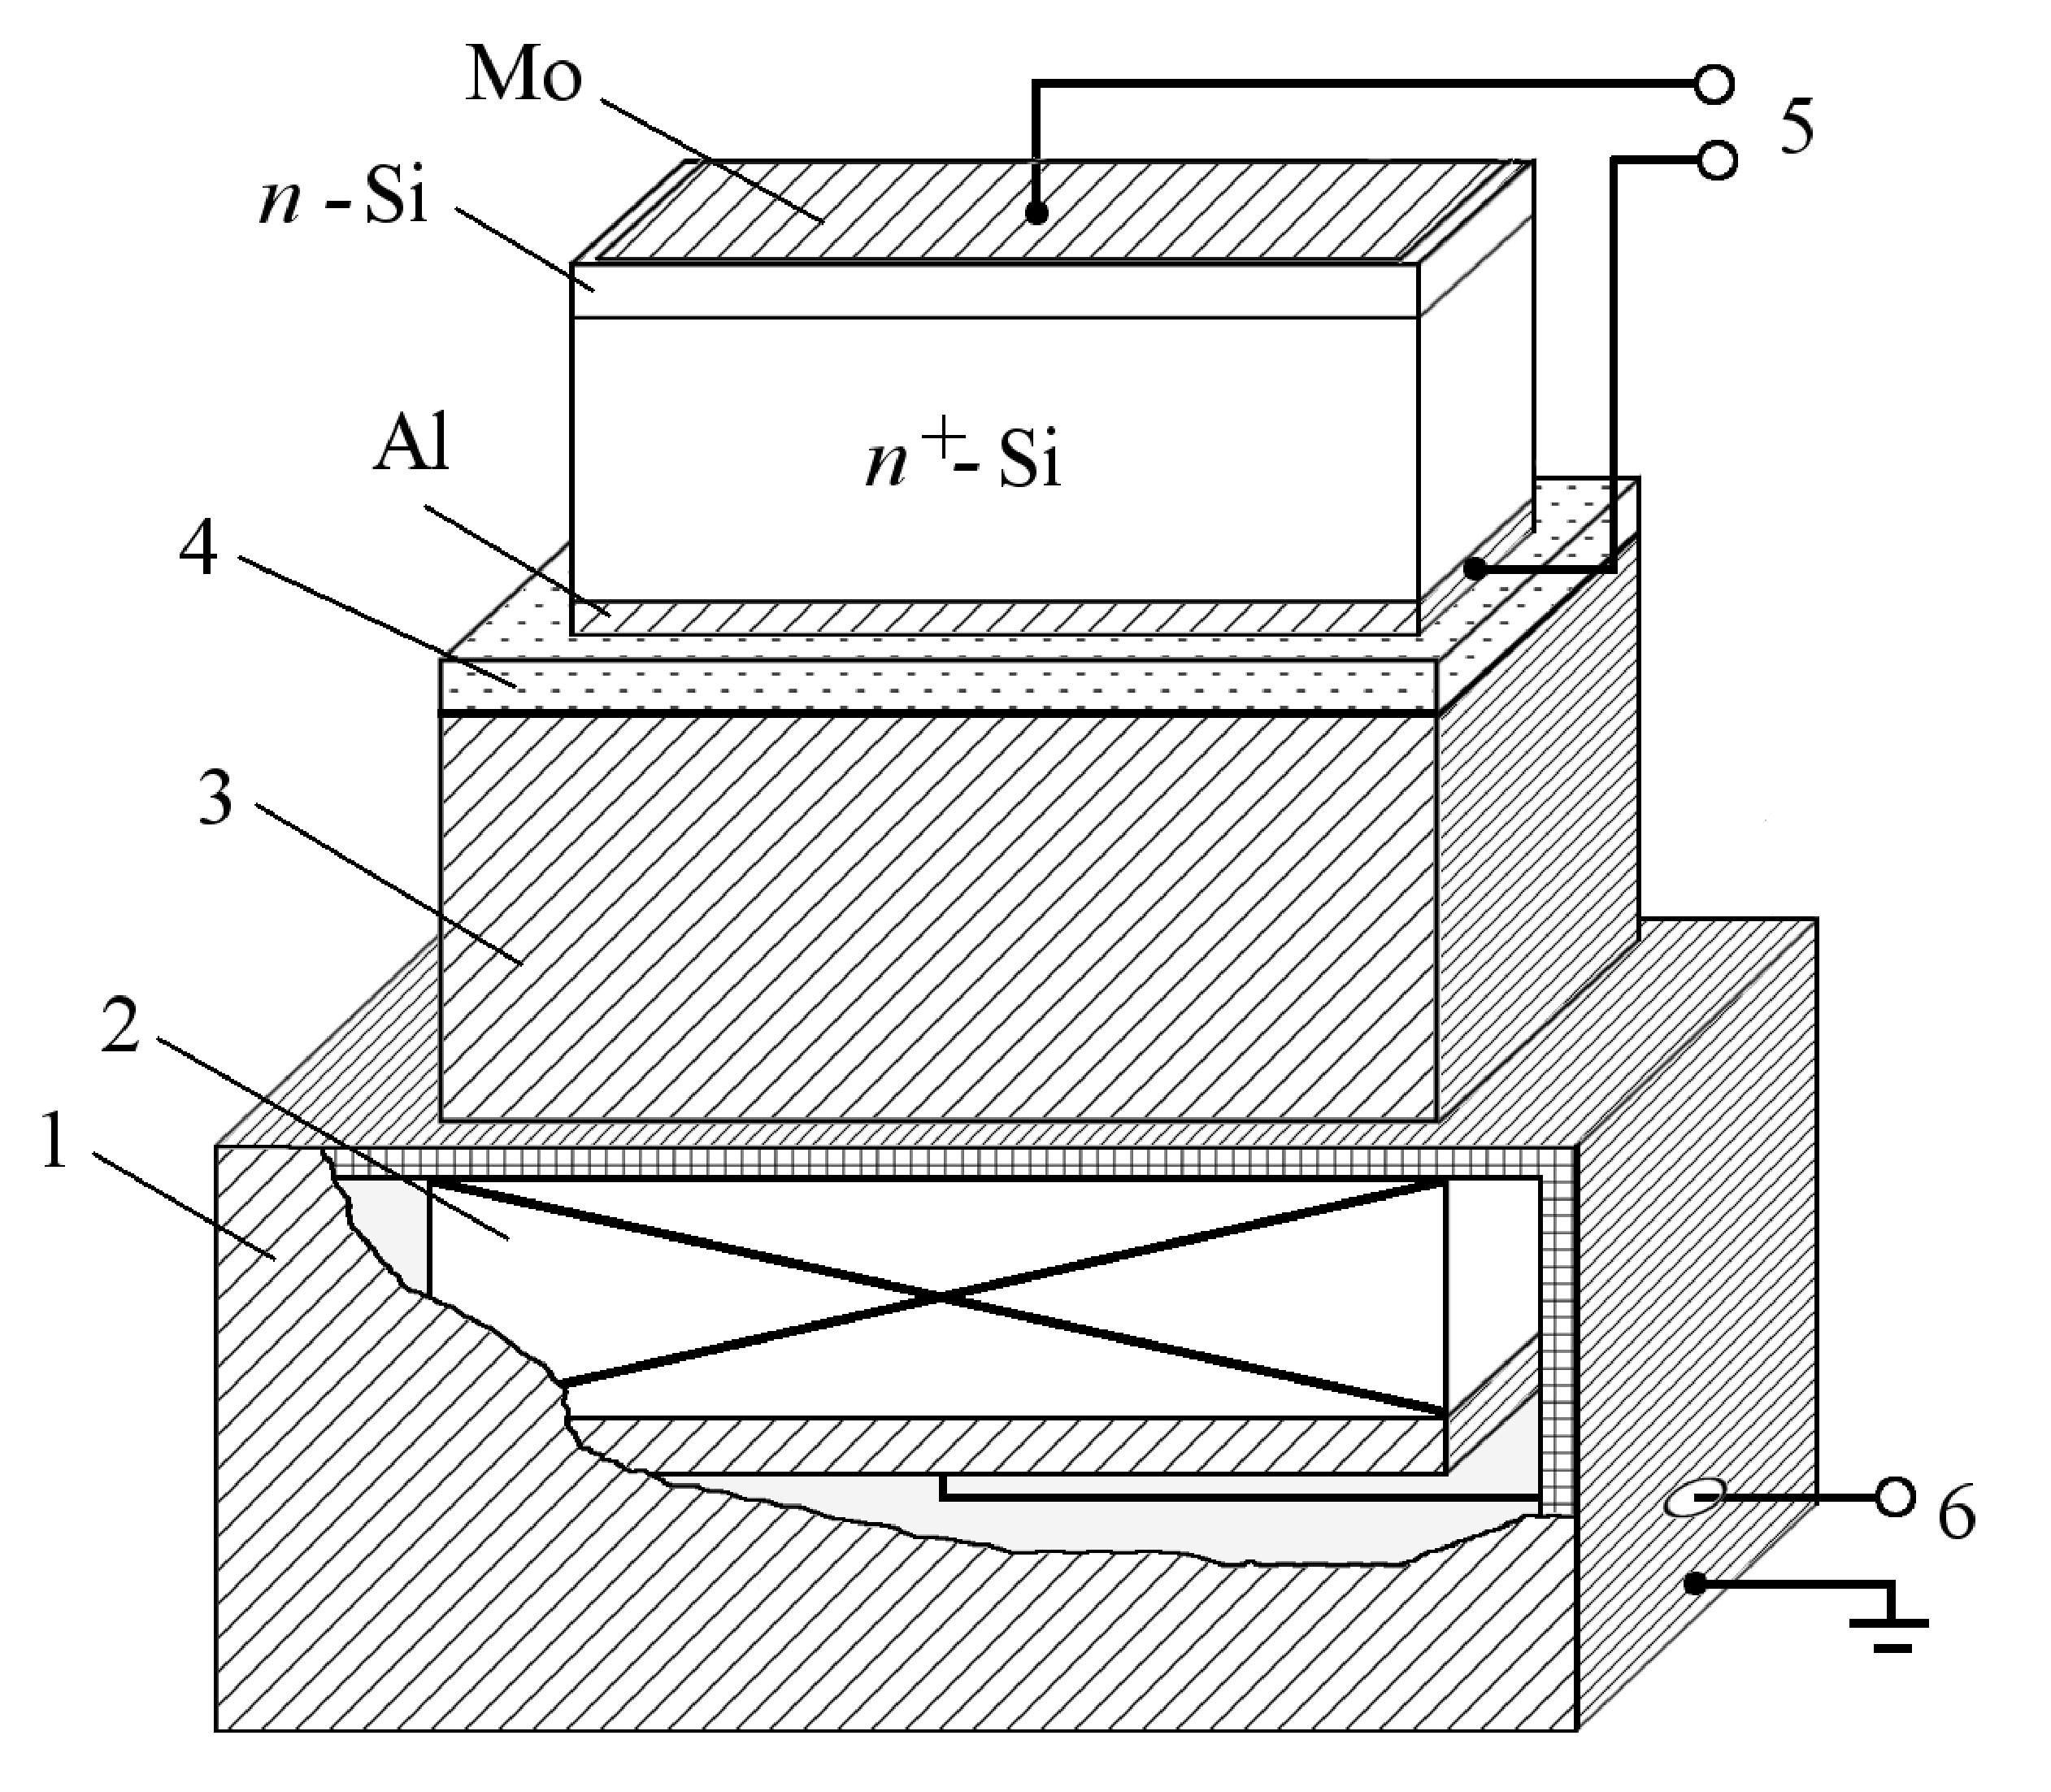
\includegraphics[width=0.5\textwidth]{USL_SDB}%
\caption{\label{figUSL:SDB}
Використані схеми УЗН.
1 --  екран (алюмінієва фольга, товщина 0,012 мм);
2 --- п'єзоелектричний перетворювач (LiNbO$_3$);
3 --- буфер (циліндр Al з високим ступенем паралельності граней, довжина 2~см);
4 --- діелектричний прошарок (слюда, товщина 0,03 мм);
5 --- контакти для вимірювання ВАХ;
6 --- контакти для збудження УЗ.
}
\end{figure}


Для створення акустичного контакту при різних УЗН використовувалися вакуумне масло, клей БФ6, піцеїн.
Зауважимо, що у випадку низькотемпературного (при $T<230$~К) УЗН процес збудження АХ був утруднений через те, що
рідкі акустичні склейки на кшталт вакуумного масла кристалізувалися і переставали виконувати свою функцію.
В той же час, контакт створений при кімнатній температурі за допомогою жорсткої склейки (піцеїн або БФ6),
руйнувався при охолодженні внаслідок різниці коефіцієнтів теплового розширення.
В роботі проведення низькотемпературних УЗН при використанні повздовжніх хвиль здійснювалось за допомогою свіжого (до 5~год після нанесення) контакту з клею БФ6, який ще не висох.
Наявність акустичного контакту контролювалася за виглядом залежності повного опору перетворювача від частоти (АЧХ, амплітудно--частотної характеристики).
%Зокрема, при використанні схеми, зображеної на Рис.~\ref{figUSL},в, за наявності акустичного контакту на АЧХ з'являвся ряд максимумів, пов'язаних з відбиванням хвиль від граней буфера.



\section*{Висновки до розділу \ref{Ch_USL_T_SD}}
\addcontentsline{toc}{section}{Висновки до розділу \ref{Ch_USL_T_SD}}
  \begin{enumerate}
     \item Проведено
  \end{enumerate}	

Основні результати даного розділу представлені в роботах \cite{Olikh:Rev,6CPFCS}.
